\section{Generalizations}
Up until now, we have made the assumption that a squirrel who
eats nothing dies, and that a squirrel who has at least one cached nut
(that is, $\betahat \ge 1$) will survive. It hasn't mattered so much what
the exact sequence of events is, but the generalizations to follow necessitate a bit
more delicacy. We impose that $n_t$ (the distribution of squirrels at different
levels of nuts) is observed at midnight each night. At 6am, the death event occurs. By
5pm, the squirrels have foraged for their nuts, and by 9pm have made their decision to
save or consume, and also produced any resultant offspring. 
 \\

\begin{center}
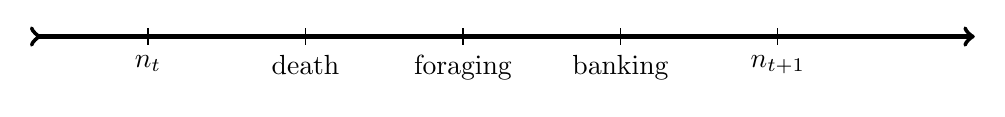
\begin{tikzpicture}
    \centering
    \draw[ultra thick, >->] (0.5,0) -- (12.5,0);
    \foreach  \x in {2, 4, 6, 8, 10}
    \draw (\x cm, 3pt) -- (\x  cm, -3pt);
    \draw[ultra thick] (2,0) node[below=3pt,thick] {$n_t$};
    \draw[ultra thick] (4,0) node[below=3pt,thick] {death};
    \draw[ultra thick] (6,0) node[below=3pt,thick] {foraging};
    \draw[ultra thick] (8,0) node[below=3pt,thick] {banking};
    \draw[ultra thick] (10,0) node[below=3pt,thick] {$n_{t+1}$};
    
\end{tikzpicture}
\end{center}

Let
\begin{itemize}
    \item $s_0, s_1, s_2, \ldots \in [0, 1]$; and
    \item $b_0, b_1, b_2, \ldots \in \left[ 0, 1 \right],$ with $\betahat := \min\left\{ k : b_k = 1 \right\}$. 
\end{itemize}
We interpret $s_k$ as the probability of surviving the night when a squirrel sleeps with cache
at $\beta = k$. Similarly, $b_k$ is the probability of using additional nuts in favour of producing
offspring rather than banking when $\beta = k$. We remark:
\begin{center}
    \textbf{$s_k$ is a variable over which squirrels have no choice, whereas $b_k$ \\
        can be viewed as a squirrel's decision to reproduce or not.}
\end{center}



\subsection{The Leslie matrix}
We ask about the fluctuation in the structure of a population of squirrels with fixed $s_k, b_k$, under
the additional hypthesis that $\pi = 2$ every day and for every squirrel. To
understand, we consider the matrix
$$ L_b = 
\begin{pmatrix}
    2s_0b_0 & s_1b_1 & s_2b_2 & \cdots & s_{\betahat - 1}b_{\betahat - 1} & s_{\betahat}b_{\betahat} \\
    s_0\left( 1-b_0 \right) & s_1b_1 & 0 & \cdots & 0 & 0 \\
    0 & s_1\left( 1-b_1 \right) & s_2b_2 & \cdots & 0 & 0 \\
    & & \ddots & \ddots & \vdots & \vdots \\
    0 & 0 & 0 & \cdots & s_{\betahat - 1}\left(1-b_{\betahat-1}\right) & s_{\betahat}b_{\betahat} \\
\end{pmatrix}.
$$
The fitness of such a squirrel population will be given by the unique positive eigenvalue of $L_b$;
how to compute said eigenvalue is not immediate to me. For now, look at squirrels who make banking/birth
decisions deterministically. That means $b_k$ = 0 for $k<\betahat$. 
In this special case,
$$ L = 
\begin{pmatrix}
    0 & 0 & 0 & \cdots & 0 & s_{\betahat} \\
    s_0 & 0 & 0 & \cdots & 0 & 0 \\
    0 & s_1 & 0 & \cdots & 0 & 0 \\
    0 & 0 & s_2 & \cdots & 0 & 0 \\
    \vdots & \vdots & \vdots & \ddots & \vdots & \vdots \\
    0 & 0 & 0 & \cdots & s_{\betahat - 1} & s_{\betahat} \\
\end{pmatrix}
$$
One can do some clever analysis (I'll fill this in later) to find that that the characteristic polynomial for
$L$ in $\lambda$ is
$$ \lambda^{\betahat + 2} - s_{\betahat}\lambda^{\betahat+1} - \prod\limits_{k = 0}^{\betahat} s_k = 0. $$

\subsection{Limiting frequency of time spent at $\betahat$ argument}
We can intuitively argue that for birth distributions of the form $b = [0, 0, \ldots, 0, 1]$, there must
exist some optimal $\betahat$. The form of the characteristic polynomial (which gives the eigenvalue)
implies that for $r$ to increase as $\betahat$ increases, we require $s_0 < s_1 < s_2 < \ldots$. Intuitively,
it makes sense that eventually, the added cost of banking more and more nuts outweighs the benefits. A squirrel
with $10^{100}$ nuts will be fairly encumbered by keeping track of them, for instance. Thus eventually 
$s_k \ge s_{k+1} \ge s_{k+2} \ge \ldots$, so that (denoting $r_i = r|_{\betahat = i}$) we need only compare
$r_0, r_1, \ldots, r_k$ and take the $\betahat$ which maximizes. Thus $b = \left[ 0, 0, \ldots, 0, 1_{\betahat} \right]$
is the best strategy among the simple class of strategies in which squirrels save up to a given level, and then immediately
consume all additional findings toward the aim of producing offspring. \\ 

I am now hopeful to present a framework which generalizes the above so that we can conclude $b = \left[ 0, \ldots, 0, 1 \right]$ is
optimal amongst \textit{all} birth distributions $b = \left[ b_0, b_2, \ldots \right]$. Let $\phi_k$ denote the proportion of time
a squirrel spends at cache level $\beta = k$. Then, of course $\phi_k$ is a random variable, and the vector 
$\left( \phi_0,\phi_1, \phi_2, \ldots \right)$ is a random vector which sums to 1. So $E\phi_k$ is well defined, and I propose the following:
fitness $r$ is optimized if and only if $E\phi_{\betahat}$ is optimized, where $\betahat$ is the cache level optimizing among strategies
of the form $b = [0, 0, \ldots, 0, 1]$. 

\section{QUESTIONS/COMMENTS}

\begin{itemize}
    \item I feel like $b = \left( 0, 0, \ldots, 0, 1_{\betahat} \right)$ will lead to optimal population
        growth rate. Is this so? How can I prove it?
    \item Back to the distinction between saving for a rainy day and deciding to consume now rather than later.
        It seems to me that all of the analysis to this point helps to answer the question: (how much) should I save
        for a rainy day? To understand intertemporal discounting, one will have to offer squirrels a certain amount
        of nuts right now and compare it with how many nuts must be offered in the future to compensate for the delay.
        Normally, one looks at utility. Here, it seems to me that fitness is our stand-in for utility. 
\end{itemize}


